% =====================================================================
%  Capítulo 21. Proyecto integrador
% =====================================================================
\chapter[Proyecto integrador]{Proyecto integrador: riesgo y asignación de una cartera de acciones tecnológicas}\label{cap:proyecto}

\section*{Objetivos de aprendizaje}
Al terminar este capítulo, el lector podrá:
\begin{enumerate}[label=\arabic*.,leftmargin=*]
  \item Organizar un análisis econométrico financiero completo, de la pregunta al informe, con código reproducible en
        R y en Python.
  \item Encadenar los métodos del libro: hechos estilizados, modelos de factores, volatilidad condicional, medidas de
        riesgo y asignación de cartera.
  \item Separar con rigor la estimación de la evaluación fuera de muestra y reconocer los sesgos que invalidan un
        análisis: la información del futuro, la selección de la muestra y las pruebas múltiples.
  \item Redactar conclusiones que distingan lo que los datos muestran de lo que no pueden mostrar.
\end{enumerate}

\section*{Motivación}
Los capítulos anteriores presentaron cada método por separado. En la práctica, un analista recibe una pregunta y debe
decidir qué métodos usar, en qué orden y cómo evaluar el resultado. Este capítulo resuelve un caso completo: un comité de
inversiones considera una cartera de cuatro grandes acciones tecnológicas estadounidenses y pide responder cinco preguntas.
¿Cómo se comportan sus rendimientos? ¿Cuánto riesgo de mercado agregan? ¿Cómo pronosticar su volatilidad? ¿Cuánto puede
perder la cartera en un mal día, y son confiables esas cifras? ¿Conviene ponderar por igual o minimizar la varianza?

\paragraph{Datos del capítulo.} Precios de cierre diarios ajustados de Apple (AAPL), Amazon (AMZN), Facebook (FB) y
Alphabet (GOOG), y el índice S\&P 500, del 2 de enero de 2014 al 31 de diciembre de 2018 (1\,257 rendimientos diarios), los
mismos del Capítulo~\ref{cap:eventos}. El índice es de precios: no incluye dividendos.

% ---------------------------------------------------------------------
\section{Un flujo de trabajo reproducible}
% ---------------------------------------------------------------------

Un proyecto empírico sigue cinco pasos, y cada uno tiene un error típico que el libro ha señalado.
\begin{enumerate}[label=\arabic*.,leftmargin=*]
  \item \textbf{Pregunta y datos.} Definir qué decisión informa el análisis y qué datos la responden. Documentar la fuente, la
        fecha de descarga y cada transformación (el archivo \texttt{FUENTES.txt} del proyecto). \emph{Error típico}: usar datos
        con sesgo de supervivencia o sin ajustar por dividendos y divisiones.
  \item \textbf{Diagnóstico.} Describir los datos antes de modelarlos: momentos, colas, autocorrelación de los rendimientos y de sus
        cuadrados. \emph{Error típico}: suponer normalidad o independencia sin verificarlas.
  \item \textbf{Modelo y estimación.} Elegir el modelo más simple que capture los rasgos encontrados y estimarlo con datos de una
        ventana de estimación. \emph{Error típico}: elegir el modelo después de ver su desempeño en los datos de evaluación.
  \item \textbf{Evaluación fuera de muestra.} Medir el desempeño con datos que no intervinieron en la estimación ni en la elección
        del modelo, con las pruebas adecuadas (Kupiec y Christoffersen para el VaR; Diebold-Mariano para pronósticos). \emph{Error
        típico}: usar en el pronóstico de $t$ información posterior a $t$.
  \item \textbf{Informe.} Responder la pregunta con cifras, incertidumbre y limitaciones. \emph{Error típico}: informar solo
        los resultados significativos.
\end{enumerate}
La Figura~\ref{fig:flujo} muestra cómo se encadenan las cinco etapas del proyecto y qué capítulos usa cada una. Todo el código
reutiliza las funciones ya escritas: \texttt{cap08\_funciones} para el GARCH y \texttt{cap13\_funciones} para el VaR, el ES y las
pruebas retrospectivas.

\begin{figure}[ht]
\centering
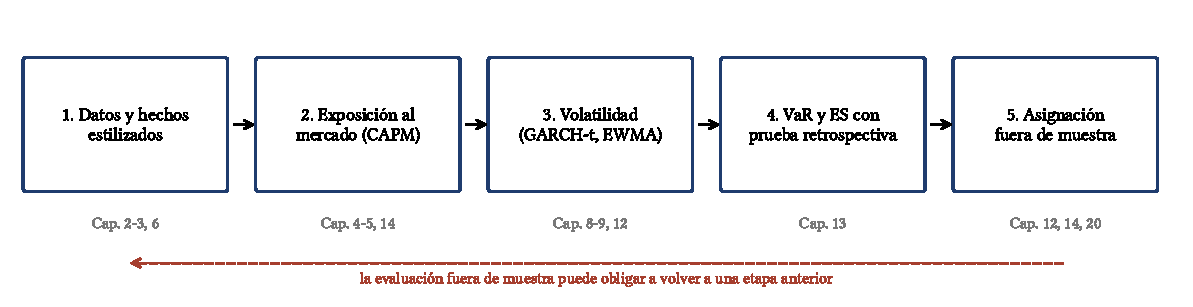
\includegraphics[width=\linewidth]{graficos/cap21_fig_flujo.pdf}
\caption{Etapas del proyecto integrador y capítulos del libro que usa cada una.}
\label{fig:flujo}
\end{figure}

% ---------------------------------------------------------------------
\section{Herramientas adicionales para el proyecto}
% ---------------------------------------------------------------------

La primera herramienta es la cartera de mínima varianza global de la Proposición~\ref{prop:minvar} (Capítulo~\ref{cap:dcc}):
\[
  \mathbf w^*=\frac{\Sigma^{-1}\mathbf 1}{\mathbf 1'\Sigma^{-1}\mathbf 1},\qquad \sigma^2_{\min}=\frac{1}{\mathbf 1'\Sigma^{-1}\mathbf 1}.
\]

La cartera de mínima varianza solo necesita covarianzas, no medias, y por eso se estima mejor que la cartera tangente: los
rendimientos esperados son la parte más ruidosa (Merton, 1980). Aun así, con $\Sigma$ estimada, $\mathbf w^*$ hereda el error de
estimación. DeMiguel, Garlappi y Uppal (2009) mostraron que la regla ingenua $1/N$, que no estima nada, es difícil de superar
fuera de muestra.

\begin{proposicion}[Error estándar de la razón de Sharpe]\label{prop:sesharpe}
Si los rendimientos son i.i.d.\ normales con media $\mu$ y desviación $\sigma$, la razón de Sharpe muestral
$\widehat{SR}=\bar r/\hat\sigma$ con $T$ observaciones cumple, aproximadamente,
\[
  \Var(\widehat{SR})\approx\frac{1}{T}\Bigl(1+\frac{SR^2}{2}\Bigr).
\]
\end{proposicion}

\begin{proof}
Con normalidad, $\bar r$ y $\hat\sigma^2$ son independientes, $\Var(\bar r)=\sigma^2/T$ y $\Var(\hat\sigma^2)\approx2\sigma^4/T$. Por el método delta,
con $g(m,v)=m/\sqrt v$, $\partial g/\partial m=1/\sigma$ y $\partial g/\partial v=-\mu/(2\sigma^3)$:
\begin{align*}
  \Var(\widehat{SR}) &\approx \Bigl(\frac1\sigma\Bigr)^2\frac{\sigma^2}{T}+\Bigl(\frac{\mu}{2\sigma^3}\Bigr)^2\frac{2\sigma^4}{T}\\
                     &= \frac1T+\frac{\mu^2}{4\sigma^6}\cdot\frac{2\sigma^4}{T}\\
                     &= \frac1T+\frac{\mu^2}{2\sigma^2T}\\
                     &= \frac1T\Bigl(1+\frac{SR^2}{2}\Bigr).
\end{align*}
\end{proof}

Con datos diarios, $SR$ es pequeño y el error estándar es casi $1/\sqrt T$. Anualizado (multiplicando por $\sqrt{252}$), con cuatro años de
datos es cercano a $\sqrt{252/1\,007}=0{,}50$: una razón de Sharpe anual de 1 no es distinguible de 0 con 95\,\% de confianza (Lo, 2002).

\begin{proposicion}[Pruebas múltiples]\label{prop:multiples}
Si se prueban $K$ hipótesis nulas verdaderas e independientes, cada una al nivel $\alpha$, la probabilidad de al menos un rechazo es
$1-(1-\alpha)^K$. Con la corrección de Bonferroni (nivel $\alpha/K$ en cada prueba) esa probabilidad es como máximo $\alpha$.
\end{proposicion}

\begin{proof}
La probabilidad de no rechazar ninguna es el producto de las de no rechazar cada una:
\begin{align*}
  \Pr(\text{ningún rechazo}) &= \prod_{k=1}^K(1-\alpha)\\
                             &= (1-\alpha)^K,\\
  \Pr(\text{al menos uno}) &= 1-(1-\alpha)^K .
\end{align*}
Para Bonferroni, por la desigualdad de Boole y sin necesidad de independencia:
\begin{align*}
  \Pr\Bigl(\bigcup_k\{\text{rechazo }k\}\Bigr) &\le \sum_{k=1}^K\Pr(\text{rechazo }k)\\
                                             &= K\cdot\frac{\alpha}{K}\\
                                             &= \alpha .
\end{align*}
\end{proof}

Con 20 estrategias sin valor, cada una al 5\,\%, la probabilidad de encontrar al menos una ``significativa'' es $1-0{,}95^{20}=0{,}64$. Es el
problema de la minería de datos (Harvey, Liu y Zhu, 2016). Un caso extremo es la \emph{selección de la muestra}: elegir hoy los activos que
mejor rindieron en el pasado garantiza que su rendimiento pasado parezca extraordinario.

% ---------------------------------------------------------------------
\section{El proyecto, etapa por etapa}
% ---------------------------------------------------------------------

\begin{ejresuelto}{Etapa 1: los datos y sus hechos estilizados}\label{ej:etapa1}
\enunciado Describa los cinco rendimientos diarios: media y volatilidad anualizadas, asimetría, curtosis, prueba de Jarque-Bera,
Ljung-Box de 10 rezagos para los rendimientos y sus cuadrados, peor día y correlaciones.

\solucion
\paso{Paso 1. Momentos.}
\begin{center}\small
\begin{tabular}{@{}lrrrrrrr@{}}
\toprule
Serie & Media anual & Vol.\ anual & Asimetría & Curtosis & JB & LB($r^2$) & Peor día \\
\midrule
AAPL & 19,99 & 24,04 & $-0{,}05$ & 6,67 & 707 & 52,9 & $-7{,}99$ \\
AMZN & 31,41 & 30,99 & 0,50 & 12,55 & 4\,824 & 22,9 & $-11{,}00$ \\
FB & 22,02 & 29,92 & $-0{,}18$ & 18,21 & 12\,125 & 11,5 & $-18{,}96$ \\
GOOG & 15,31 & 23,45 & 0,96 & 15,96 & 8\,990 & 17,1 & $-5{,}32$ \\
S\&P 500 & 7,16 & 13,23 & $-0{,}43$ & 6,74 & 770 & 386,0 & $-4{,}10$ \\
\bottomrule
\end{tabular}
\end{center}
Todas las series rechazan la normalidad con holgura (valor crítico de JB al 1\,\%: 9,21). Ninguna tiene autocorrelación significativa al 1\,\% en los
rendimientos (valor crítico 23,21). En los cuadrados, el S\&P 500 (386,0) y Apple (52,9) muestran un agrupamiento de volatilidad muy fuerte; Facebook
no (11,5): sus días extremos son saltos aislados por noticias propias, como la caída del 26 de julio de 2018 del Capítulo~\ref{cap:eventos}.

\paso{Paso 2. Dependencia.} Las correlaciones entre las acciones van de 0,40 (AAPL-FB) a 0,62 (AMZN-GOOG), y con el S\&P 500, de 0,56 a 0,67
(Figura~\ref{fig:riqueza}).

\paso{Paso 3. Una advertencia sobre la muestra.} Estas cuatro empresas se eligen hoy porque fueron las grandes ganadoras de la década: con
medias anuales de 15 a 31\,\%, frente a 7\,\% del índice. Cualquier conclusión sobre su rendimiento medio tiene \emph{sesgo de selección}. Por eso
el proyecto se concentra en el riesgo, que depende de varianzas y correlaciones y es mucho menos sensible a esa elección.

\codigoweb{cap21_ej01}
\salidaR{cap21_ej01_R.txt}
\lectura{cap21_ej01}

\RvsPy El archivo de funciones del proyecto importa las de los Capítulos 8 y 13 (\texttt{source} en R, \texttt{from ... import} en Python), de modo que el
GARCH y las pruebas retrospectivas son exactamente las ya verificadas. El estadístico de Ljung-Box se programa directamente para controlar la
definición de las autocorrelaciones.

\begin{figure}[ht]
\centering
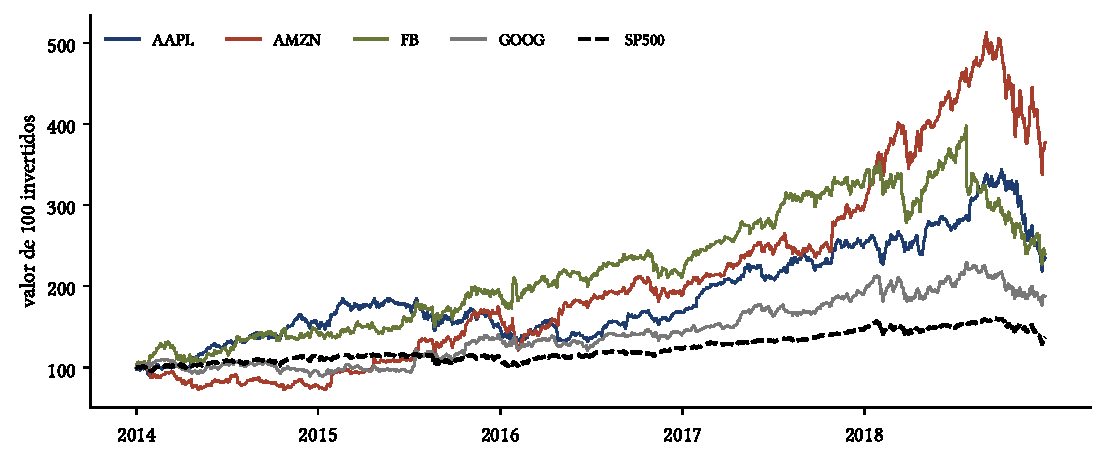
\includegraphics[width=\linewidth]{graficos/cap21_ej01_riqueza.pdf}
\caption{Valor de 100 invertidos en cada acción y en el S\&P 500 a inicios de 2014.}
\label{fig:riqueza}
\end{figure}

\begin{conclusion}
Los rendimientos tienen colas mucho más pesadas que la normal, no son predecibles en media y, salvo Facebook, muestran agrupamiento de volatilidad. Los
modelos de riesgo deben incorporar ambos rasgos.
\end{conclusion}
\end{ejresuelto}

\begin{ejresuelto}{Etapa 2: exposición al mercado}\label{ej:etapa2}
\enunciado Estime el CAPM diario de cada acción y de la cartera 1/N con el S\&P 500 como mercado y errores de Newey-West de 5 rezagos.

\solucion
\paso{Paso 1. Betas y alfas.}
\begin{center}\small
\begin{tabular}{@{}lrrrrr@{}}
\toprule
Acción & Alfa anual (\%) & $t$(alfa) & Beta & $t$(beta $=1$) & $R^2$ \\
\midrule
AAPL & 11,91 & 1,34 & 1,127 & 2,88 & 0,384 \\
AMZN & 21,79 & 1,96 & 1,343 & 4,36 & 0,329 \\
FB & 13,03 & 1,23 & 1,255 & 4,79 & 0,308 \\
GOOG & 6,78 & 0,89 & 1,190 & 4,55 & 0,451 \\
Cartera 1/N & 13,38 & 2,23 & 1,229 & -- & 0,566 \\
\bottomrule
\end{tabular}
\end{center}
Las cuatro betas son significativamente mayores que 1: la cartera amplifica los movimientos del mercado en un 23\,\%. La beta de la cartera es el promedio
de las betas, como debe ser por linealidad. Entre el 55 y el 69\,\% de la varianza de cada acción es idiosincrática, y la diversificación entre solo cuatro
acciones la reduce: el $R^2$ de la cartera sube a 0,57.

\paso{Paso 2. El alfa.} El alfa de la cartera, 13,4\,\% anual con $t=2{,}23$, sería significativo al 5\,\% si fuera la única prueba. Pero con cinco pruebas
(Proposición~\ref{prop:multiples}) el nivel de Bonferroni es $0{,}05/5=0{,}01$, y sobre todo la muestra se eligió por su rendimiento pasado: el alfa es,
en buena medida, el sesgo de selección de la Etapa 1. No es una predicción.

\paso{Paso 3. Estabilidad.} La beta de la cartera sube de 1,185 en 2014--2015 a 1,261 en 2016--2018.

\codigoweb{cap21_ej02}
\salidaR{cap21_ej02_R.txt}
\lectura{cap21_ej02}

\RvsPy Usamos rendimientos totales en lugar de excesos: la tasa libre de riesgo diaria entre 2014 y 2018 fue de pocas milésimas de punto porcentual y no
altera las betas. Los errores de Newey-West usan la función \texttt{nw\_mco} del proyecto, la misma fórmula del Capítulo~\ref{cap:robustos}.

\begin{conclusion}
La cartera es un instrumento de mercado amplificado: su riesgo está dominado por el del mercado (beta de 1,23) y la diversificación entre cuatro acciones
correlacionadas es limitada.
\end{conclusion}
\end{ejresuelto}

\begin{ejresuelto}{Etapa 3: pronóstico de la volatilidad}\label{ej:etapa3}
\enunciado Estime un GARCH(1,1) con errores $t$ para cada serie con los datos de 2014--2015. Sin reestimar, filtre la varianza día a día en 2016--2018 y
compare sus pronósticos con los de EWMA ($\lambda=0{,}94$) y una varianza constante, con las pérdidas QLIKE ($\ln h_t+e_t^2/h_t$) y cuadrática (Patton, 2011), y la
prueba de Diebold-Mariano.

\solucion
\paso{Paso 1. Estimaciones} (2014--2015, 503 días).
\begin{center}\small
\begin{tabular}{@{}lrrrrr@{}}
\toprule
Serie & $\alpha$ & $\beta$ & $\nu$ & $\alpha+\beta$ & Vida media (días) \\
\midrule
AAPL & 0,065 & 0,862 & 4,76 & 0,927 & 9,2 \\
AMZN & 0,000 & 0,991 & 3,33 & 0,991 & 75,6 \\
FB & 0,014 & 0,971 & 6,30 & 0,985 & 44,7 \\
GOOG & 0,142 & 0,619 & 4,87 & 0,760 & 2,5 \\
S\&P 500 & 0,213 & 0,719 & 7,80 & 0,932 & 9,8 \\
\bottomrule
\end{tabular}
\end{center}
Con solo dos años de datos, las estimaciones de las acciones individuales son inestables: en Amazon, $\alpha$ queda en la frontera (cero) y la varianza
casi no reacciona a los choques. Los grados de libertad, entre 3,3 y 7,8, confirman las colas pesadas. La vida media se calcula como
\begin{align*}
  h_{1/2} &= \frac{\ln0{,}5}{\ln(\alpha+\beta)}\\
          &= \frac{-0{,}6931}{\ln0{,}9319}\\
          &= \frac{-0{,}6931}{-0{,}0705}\\
          &= 9{,}8\ \text{días}
\end{align*}
para el S\&P 500.

\paso{Paso 2. Evaluación fuera de muestra} (754 días).
\begin{center}\small
\begin{tabular}{@{}lrrrr@{}}
\toprule
Serie & QLIKE GARCH-$t$ & QLIKE EWMA & QLIKE constante & DM (GARCH $-$ EWMA) \\
\midrule
AAPL & 1,699 & 1,807 & 1,801 & $-1{,}29$ \\
AMZN & 2,246 & 2,205 & 2,266 & 0,17 \\
FB & 2,144 & 2,195 & 2,223 & $-0{,}57$ \\
GOOG & 1,560 & 1,542 & 1,684 & 0,34 \\
S\&P 500 & 0,249 & 0,352 & 0,605 & $-1{,}40$ \\
\bottomrule
\end{tabular}
\end{center}
Los dos modelos dinámicos superan a la varianza constante en todas las series. Entre ellos no hay un ganador claro: GARCH-$t$ tiene menor pérdida en tres
series y EWMA en dos, pero ninguna diferencia es significativa ($|DM|<1{,}96$). EWMA, que no estima parámetros, es tan bueno como un GARCH estimado con
dos años de datos (Figura~\ref{fig:volatilidad21}).

\codigoweb{cap21_ej03}
\salidaR{cap21_ej03_R.txt}
\lectura{cap21_ej03}

\RvsPy El GARCH se estima con \texttt{nlminb} en R y con \texttt{L-BFGS-B} en Python, con las mismas condiciones del Capítulo~\ref{cap:garch}; en estos datos
ambos llegan al mismo óptimo hasta la cuarta decimal. El filtrado fuera de muestra aplica la recursión \texttt{garch\_s2} con los parámetros fijos a toda la
serie, de modo que la varianza del día $t$ usa solo los rendimientos hasta $t-1$.

\begin{figure}[ht]
\centering
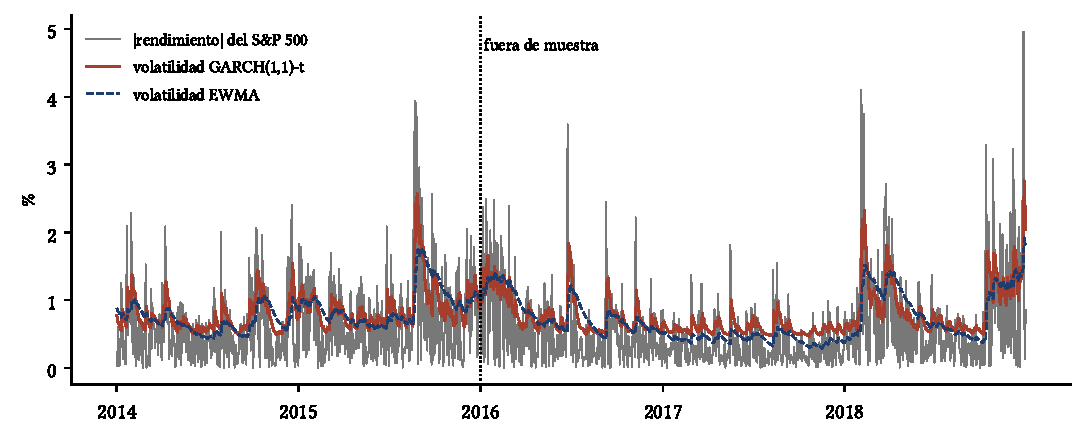
\includegraphics[width=\linewidth]{graficos/cap21_ej03_volatilidad.pdf}
\caption{Valor absoluto del rendimiento diario del S\&P 500 con las volatilidades GARCH(1,1)-$t$ y EWMA. A la derecha de la línea punteada, los parámetros del
GARCH están fijos en los estimados con 2014--2015.}
\label{fig:volatilidad21}
\end{figure}

\begin{conclusion}
Para pronosticar la volatilidad diaria, cualquier modelo dinámico es mucho mejor que uno constante, y la elección entre GARCH y EWMA es secundaria. Con
muestras cortas, la simplicidad de EWMA es una ventaja.
\end{conclusion}
\end{ejresuelto}

\begin{ejresuelto}{Etapa 4: VaR y ES de la cartera}\label{ej:etapa4}
\enunciado Para la cartera 1/N, calcule el VaR y el ES diarios al 99 y al 97,5\,\% de 2016 a 2018 con simulación histórica (250 días), EWMA normal y
GARCH(1,1)-$t$ (estimado en 2014--2015 y reestimado cada enero con todos los datos anteriores). Evalúe con las pruebas de Kupiec y de Christoffersen, y
compare la pérdida media en los días de excepción con el ES pronosticado.

\solucion
\paso{Paso 1. Resultados al 99\,\%} (754 días; 7,5 excepciones esperadas).
\begin{center}\small
\begin{tabular}{@{}lrrrr@{}}
\toprule
Método & Excepciones & $p$ Kupiec & $p$ Christoffersen & Pérdida/ES \\
\midrule
Simulación histórica & 14 & 0,035 & 0,466 & 1,043 \\
EWMA normal & 21 & 0,000 & 0,611 & 1,173 \\
GARCH-$t$ (fijo) & 14 & 0,035 & 0,466 & 0,931 \\
GARCH-$t$ (reestimado) & 13 & 0,070 & 0,499 & 0,931 \\
\bottomrule
\end{tabular}
\end{center}
El EWMA normal falla con claridad: 21 excepciones, casi el triple de las esperadas, porque la normal no tiene colas suficientes. Los demás también
subestiman el riesgo, pero menos. Solo el GARCH-$t$ reestimado cada año no se rechaza al 5\,\% (13 excepciones, $p=0{,}070$). Ninguno muestra excepciones
agrupadas.

\paso{Paso 2. Al 97,5\,\%} (18,9 esperadas): las cuatro alternativas tienen entre 27 y 28 excepciones. Los dos GARCH-$t$ no se rechazan ($p=0{,}074$); la
simulación histórica falla además la prueba de independencia ($p=0{,}019$), porque reacciona tarde a los cambios de volatilidad.

\paso{Paso 3. El ES.} En los días de excepción al 99\,\%, la pérdida realizada fue en promedio 0,93 veces el ES del GARCH-$t$: el ES fue suficiente. Con EWMA
normal fue 1,17 veces: el ES normal también es corto. Al reestimar con toda la muestra ($\alpha=0{,}141$, $\beta=0{,}831$, $\nu=4{,}34$), el pronóstico para el
primer día hábil de 2019, después de un diciembre de 2018 muy volátil, es una volatilidad de 2,87\,\%, un VaR al 99\,\% de 7,42\,\% y un ES de 10,18\,\%
(Figura~\ref{fig:var21}).

\codigoweb{cap21_ej04}
\salidaR{cap21_ej04_R.txt}
\lectura{cap21_ej04}

\RvsPy La reestimación anual usa en cada enero solo los datos de los años anteriores y filtra la varianza del año con esos parámetros. En R los
parámetros de cada día se guardan en una matriz indexada por fecha; en Python, en un diccionario. La simulación histórica del día $t$ usa las pérdidas
de $t-250$ a $t-1$.

\begin{figure}[ht]
\centering
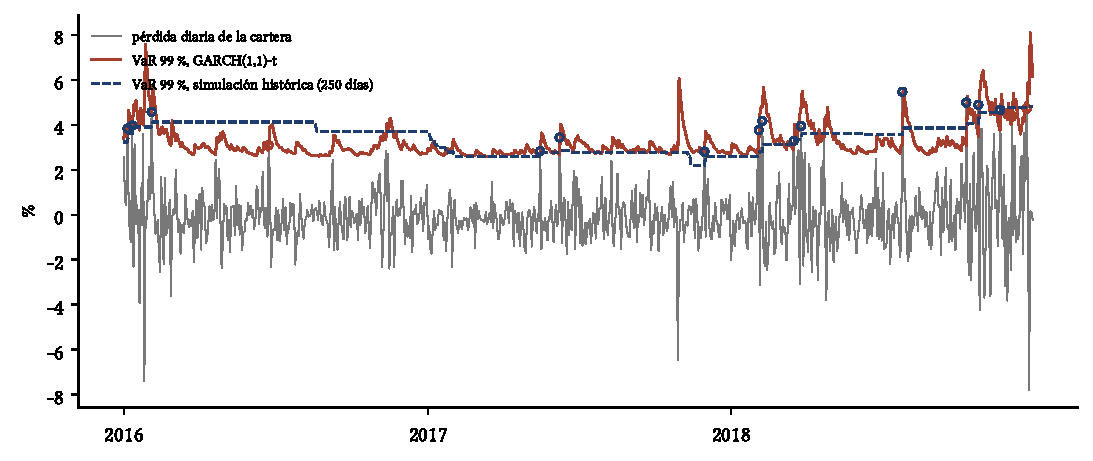
\includegraphics[width=\linewidth]{graficos/cap21_ej04_var.pdf}
\caption{Pérdida diaria de la cartera 1/N con el VaR al 99\,\% del GARCH(1,1)-$t$ fijo y de la simulación histórica, y sus excepciones (círculos).}
\label{fig:var21}
\end{figure}

\begin{conclusion}
Las colas pesadas importan más que la dinámica: la normal falla aunque su volatilidad sea dinámica. La recomendación al comité es un GARCH con errores $t$,
reestimado al menos una vez al año y con su prueba retrospectiva informada junto con la cifra de VaR.
\end{conclusion}
\end{ejresuelto}

\begin{ejresuelto}{Etapa 5: asignación fuera de muestra}\label{ej:etapa5}
\enunciado Desde enero de 2015, cada 21 días hábiles, forme la cartera 1/N y la de mínima varianza global con la covarianza muestral de los últimos 250 días y
con la covarianza EWMA. Compare media, volatilidad, razón de Sharpe, máxima caída y rotación.

\solucion
\paso{Paso 1. Resultados} (1\,007 días; 48 rebalanceos).
\begin{center}\small
\begin{tabular}{@{}lrrrrr@{}}
\toprule
Estrategia & Media (\%) & Vol.\ (\%) & Sharpe & Máx.\ caída (\%) & Rotación \\
\midrule
1/N & 23,42 & 21,82 & 1,073 & 29,52 & 0,000 \\
Mínima varianza (muestral) & 17,83 & 21,63 & 0,824 & 30,13 & 0,146 \\
Mínima varianza (EWMA) & 18,41 & 22,86 & 0,805 & 36,04 & 0,990 \\
\bottomrule
\end{tabular}
\end{center}
La cartera de mínima varianza con covarianza muestral reduce la volatilidad apenas de 21,82 a 21,63\,\% anual, y con covarianza EWMA la \emph{aumenta}. El
objetivo de la estrategia, reducir el riesgo, prácticamente no se logra: con cuatro activos de correlaciones parecidas, la cartera 1/N ya está cerca de la de
mínima varianza, y el error de estimación de $\Sigma$ consume la pequeña ganancia teórica. La versión EWMA rota casi el 100\,\% de la cartera en cada
rebalanceo, y su peso mínimo es negativo en promedio ($-0{,}096$).

\paso{Paso 2. ¿Es mejor 1/N?} Su razón de Sharpe es mayor, pero por la Proposición~\ref{prop:sesharpe}, con 1\,007 días,
\begin{align*}
  \text{ee}(\widehat{SR}_{\text{anual}}) &\approx \sqrt{252}\sqrt{\frac{1+(1{,}073/\sqrt{252})^2/2}{1\,007}}\\
                                         &= 0{,}501,
\end{align*}
de modo que las tres razones de Sharpe están a menos de un error estándar entre sí. Las dos estrategias principales tienen una correlación diaria de 0,95: son
casi la misma cartera. La mínima varianza muestral pondera más a Apple (0,41) y Alphabet (0,40), las de menor volatilidad, y menos a Amazon (0,06)
(Figura~\ref{fig:asignacion}).

\codigoweb{cap21_ej05}
\salidaR{cap21_ej05_R.txt}
\lectura{cap21_ej05}

\RvsPy Los pesos se calculan con \texttt{solve(S, 1)} en ambos lenguajes en lugar de invertir $\Sigma$. Se suponen pesos constantes entre rebalanceos (rebalanceo
diario implícito) y sin costos de transacción; con costos, la ventaja de 1/N, que nunca rota, sería mayor.

\begin{figure}[ht]
\centering
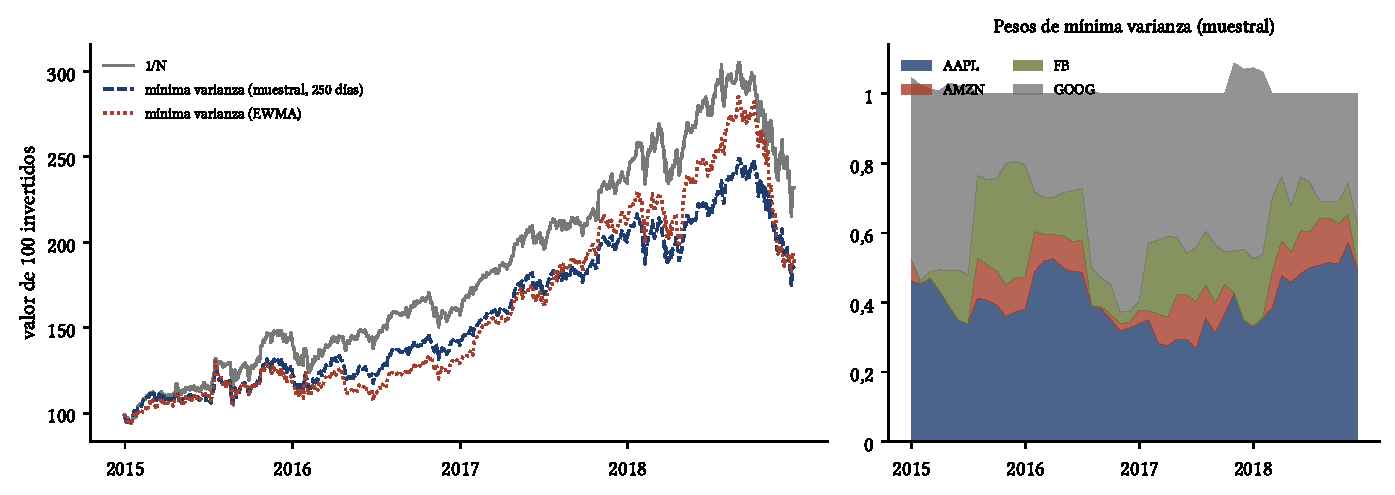
\includegraphics[width=\linewidth]{graficos/cap21_ej05_asignacion.pdf}
\caption{Izquierda: valor de 100 invertidos en cada estrategia desde enero de 2015. Derecha: pesos de la cartera de mínima varianza muestral en cada rebalanceo
(las posiciones cortas, en 12 de los 48 rebalanceos, se muestran como cero).}
\label{fig:asignacion}
\end{figure}

\begin{conclusion}
Optimizar no siempre mejora. Con pocos activos parecidos, la regla 1/N es tan buena como la de mínima varianza y no tiene costos de estimación ni de rotación,
como encontraron DeMiguel, Garlappi y Uppal (2009).
\end{conclusion}
\end{ejresuelto}

% ---------------------------------------------------------------------
\section{El informe al comité}
% ---------------------------------------------------------------------

Un informe útil responde cada pregunta en una o dos oraciones, con la cifra, su incertidumbre y la limitación principal:
\begin{enumerate}[label=\arabic*.,leftmargin=*]
  \item \textbf{Rendimientos.} Tienen colas mucho más pesadas que la normal (curtosis de 6,7 a 18,2) y volatilidad que se agrupa. Sus medias de 2014--2018
        reflejan la selección de ganadores y no deben extrapolarse.
  \item \textbf{Riesgo de mercado.} La cartera tiene una beta de 1,23 con el S\&P 500: amplifica el mercado. El alfa estimado no es evidencia de habilidad
        ni de rendimiento futuro.
  \item \textbf{Volatilidad.} Un modelo dinámico (GARCH o EWMA) es indispensable; entre ellos la diferencia no es significativa.
  \item \textbf{Pérdida máxima probable.} El VaR diario al 99\,\% para el primer día de 2019 es 7,4\,\% del valor de la cartera, y la pérdida media en el peor
        1\,\% de los días, 10,2\,\%. El modelo que lo calcula (GARCH-$t$ reestimado anualmente) pasó la prueba retrospectiva de 2016--2018 al 5\,\%, pero con
        13 excepciones frente a 7,5 esperadas: las cifras deben leerse como un mínimo.
  \item \textbf{Asignación.} Ponderar por igual es tan bueno como minimizar la varianza y más barato de mantener.
\end{enumerate}
Las limitaciones generales son tres: cinco años de datos de un período alcista, cuatro activos del mismo sector y la ausencia de costos de transacción.

% ---------------------------------------------------------------------
\section{Proyectos propuestos}
% ---------------------------------------------------------------------

\begin{enumerate}[label=\textbf{\thechapter.\arabic*},leftmargin=*,itemsep=6pt]
  \item \emph{(Cartera peruana.)} Repita el proyecto con cinco acciones de la BVL de distintos sectores (por ejemplo, minería, banca, consumo, construcción y
  energía) y el índice S\&P/BVL Perú General. ¿Cambia la conclusión sobre 1/N cuando las correlaciones son más bajas? Discuta el efecto de la negociación poco
  frecuente sobre las betas.

  \item \emph{(Sesgo de selección.)} Con los 30 carteras de French del Capítulo~\ref{cap:factores}, elija en cada enero las cuatro de mayor rendimiento en los 5 años
  anteriores y mida su rendimiento en el año siguiente. Compare con el alfa de la Etapa 2.

  \item \emph{(Cópulas.)} Sustituya en la Etapa 4 el GARCH univariado de la cartera por GARCH-$t$ marginales unidos por una cópula $t$ (Capítulo~\ref{cap:copulas}).
  ¿Mejora la prueba retrospectiva?

  \item \emph{(Regímenes.)} Estime un modelo de dos regímenes (Capítulo~\ref{cap:markov}) para los rendimientos semanales de la cartera y úselo para el VaR semanal.

  \item \emph{(Costos.)} Agregue a la Etapa 5 un costo de 10 puntos básicos por unidad de rotación. ¿Cuánto cambia la razón de Sharpe de cada estrategia?

  \item \emph{(Contracción.)} Sustituya la covarianza muestral de la Etapa 5 por la de Ledoit y Wolf (2004), que contrae hacia una matriz con correlación constante.

  \item \emph{(Evaluación del ES.)} Implemente la prueba de Acerbi y Szekely (2014) para el ES de la Etapa 4.

  \item \emph{(Informe.)} Redacte el informe al comité en no más de dos páginas, con una tabla y una figura, para un lector sin formación econométrica.
\end{enumerate}

% ---------------------------------------------------------------------
\section{Resumen de fórmulas}
% ---------------------------------------------------------------------

\begin{table}[H]
\centering\small
\begin{tabular}{@{}ll@{}}
\toprule
Concepto & Fórmula \\
\midrule
Mínima varianza global & $\mathbf w^*=\Sigma^{-1}\mathbf 1/(\mathbf 1'\Sigma^{-1}\mathbf 1)$;\quad $\sigma^2_{\min}=1/(\mathbf 1'\Sigma^{-1}\mathbf 1)$ \\
Error estándar del Sharpe & $\sqrt{(1+SR^2/2)/T}$ \\
Pruebas múltiples & $\Pr(\ge1\text{ rechazo})=1-(1-\alpha)^K$;\quad Bonferroni $\alpha/K$ \\
QLIKE & $\ln h_t+e_t^2/h_t$ \\
Vida media de la volatilidad & $\ln0{,}5/\ln(\alpha+\beta)$ \\
Rotación & $\sum_j|w_{j,k}-w_{j,k-1}|$ \\
Máxima caída & $1-\min_t V_t/\max_{s\le t}V_s$ \\
\bottomrule
\end{tabular}
\caption{Fórmulas principales del Capítulo 21.}
\end{table}

\section*{Referencias}
\begin{itemize}[leftmargin=*]
  \item Acerbi, C. y Szekely, B. (2014). Backtesting expected shortfall. \emph{Risk}, 27(11), 76--81.
  \item DeMiguel, V., Garlappi, L. y Uppal, R. (2009). Optimal versus naive diversification: How inefficient is the 1/N portfolio strategy?
        \emph{Review of Financial Studies}, 22(5), 1915--1953.
  \item Harvey, C. R., Liu, Y. y Zhu, H. (2016). \ldots\ and the cross-section of expected returns. \emph{Review of Financial Studies}, 29(1), 5--68.
  \item Ledoit, O. y Wolf, M. (2004). Honey, I shrunk the sample covariance matrix. \emph{Journal of Portfolio Management}, 30(4), 110--119.
  \item Lo, A. W. (2002). The statistics of Sharpe ratios. \emph{Financial Analysts Journal}, 58(4), 36--52.
  \item Merton, R. C. (1980). On estimating the expected return on the market: An exploratory investigation. \emph{Journal of Financial Economics},
        8(4), 323--361.
  \item Patton, A. J. (2011). Volatility forecast comparison using imperfect volatility proxies. \emph{Journal of Econometrics}, 160(1), 246--256.
\end{itemize}
